\subsection{Processamento de pacotes}
\label{sec:impl.pkt}

Nesta seção iremos mostrar como pacotes são repassados entre módulos bem
como seu conteúdo pode ser acessado para uso em tomada de decisão ou
coleta de dados.

\subsubsection{Barramento de encaminhamento}

Nosso \emph{firewall} é construído como uma extensão do projeto de placa
de rede de referência. O processamento de pacotes é realizado por uma
sequência de módulos. O \emph{firewall} é instanciado no módulo
\ssf{user\_data\_path}, que define o \emph{pipeline} de processamento,
entre os módulos \ssf{output\_port\_lookup} e \ssf{output\_queues} (ver
figura~\ref{fig:arch.pipe.iface}).

Dados dos pacotes são transmitidos entre módulos através do barramento
de encaminhamento.  Como descrito na seção~\ref{sec:arch.soft} e
ilustrado na figura~\ref{fig:arch.pipe.sinais}, o barramento de
encaminhamento é composto de 64~bits de dados (\ssf{data}), 8~bits de
controle (\ssf{ctrl}), um bit para informar que o módulo anterior tem
dado disponível para enviar (\ssf{wr}) e um bit para informar que o
módulo está pronto para receber (\ssf{rdy}).  A definição das linhas de
comunicação do barramento de encaminhamento em nosso \emph{firewall} é
mostrada abaixo:

\begin{verilogcode}
module firewall
   #(
      parameter DATA_WIDTH = 64,
      parameter CTRL_WIDTH = DATA_WIDTH/8,
      ...
   )
   (
      input [DATA_WIDTH-1:0]              in_data,
      input [CTRL_WIDTH-1:0]              in_ctrl,
      input                               in_wr,
      output                              in_rdy,
      output reg [DATA_WIDTH-1:0]         out_data,
      output reg [CTRL_WIDTH-1:0]         out_ctrl,
      output reg                          out_wr,
      input                               out_rdy,
      ...
\end{verilogcode}

Todos os módulos do \emph{pipeline} de processamento da NetFPGA, como os
módulos \ssf{output\_port\_lookup} e \ssf{output\_queues}, possuem uma
fila que armazena dados de pacotes recebidos do módulo antecessor.  A
transferência entre módulos só é realizada quando ambos sinais \ssf{wr}
e \ssf{rdy} estão ligados.  Quando o bit \ssf{wr} não está ligado, o
módulo anterior não tem dados para transferir, por exemplo, por que a
placa não recebeu nenhum pacote.  Quando o bit \ssf{rdy} não está
ligado, a fila de recepção do módulo está cheia e ele não pode receber
mais dados, por exemplo, porque o processamento de um pacote está
demorando mais do que o esperado.  Note que quando um módulo não pode
receber dados, ele pode travar todo o \emph{pipeline} de processamento.
Em nosso \emph{firewall}, a fila que armazena os dados de pacotes
transmitidas pelo módulo anterior é uma instância de
\ssf{fallthrough\_small\_fifo} chamada \ssf{input\_fifo}:

\begin{verilogcode}
   fallthrough_small_fifo #(
      ...
   ) input_fifo (
      .din           ({in_ctrl, in_data}), // Data in
      .wr_en         (in_wr),              // Write enable
      .dout          ({in_fifo_ctrl, in_fifo_data}),
      .rd_en         (in_fifo_rd_en),      // Next word
      .nearly_full   (in_fifo_nearly_full),
      .empty         (in_fifo_empty),
      ...
\end{verilogcode}

A entrada da fila, \ssf{din}, é ligada diretamente às linhas de entrada
\ssf{in\_data} e \ssf{in\_ctrl}.  O controle do recebimento de dados no
barramento de processamento é realizado em duas partes.  Primeiro,
ligamos o sinal que informa se o módulo anterior tem dados para
escrever, \ssf{in\_wr}, diretamente no controle de escrita da fila,
\ssf{wr\_en} (linha 5).  Segundo, ligamos o sinal que informa se nosso
módulo pode receber dados, \ssf{in\_rdy}, diretamente no sinal que
informa se a fila está quase cheia (apenas uma posição livre):

\begin{verilogcode}
      assign in_rdy = !in_fifo_nearly_full;
\end{verilogcode}

Se o módulo anterior não tiver dados para enviar ou se a fila estiver
cheia, nada é escrito na fila.  Mais precisamente, se a fila estiver
cheia, nada será escrito na fila e o módulo anterior irá armazenar o
dado até a fila poder recebê-lo.

Como veremos na subseção seguinte, nosso \emph{firewall} retira dados da
fila lendo os dados em \ssf{in\_fifo\_data} e \ssf{in\_fifo\_ctrl},
ligados à saída da fila (\ssf{dout}), e ligando o sinal
\ssf{in\_fifo\_rd\_en} para avançar a fila para a próximo dado.

Os bits de controle, \ssf{in\_fifo\_ctrl}, especificam como os bits de
dados devem ser processados.  Os bits de controle possuem valor zero
enquanto o pacote está sendo transmitido.  Bits de controle diferentes
de zero denotam metadados que precedem ou sucedem os dados do pacote.  O
valor dos bits de controle define a semântica dos bits de dados,
\ssf{in\_fifo\_data}.  Por exemplo, quando os bits de controle valem
\ssf{IO\_QUEUES\_STAGE\_NUM} (\ssf{0xff}), os bits de dados contém
informações sobre o recebimento do pacote, por exemplo, em qual porta
Ethernet ele chegou.  Estes metadados podem ser utilizados no
processamento do pacote.

% \begin{figure}
% \centering
% 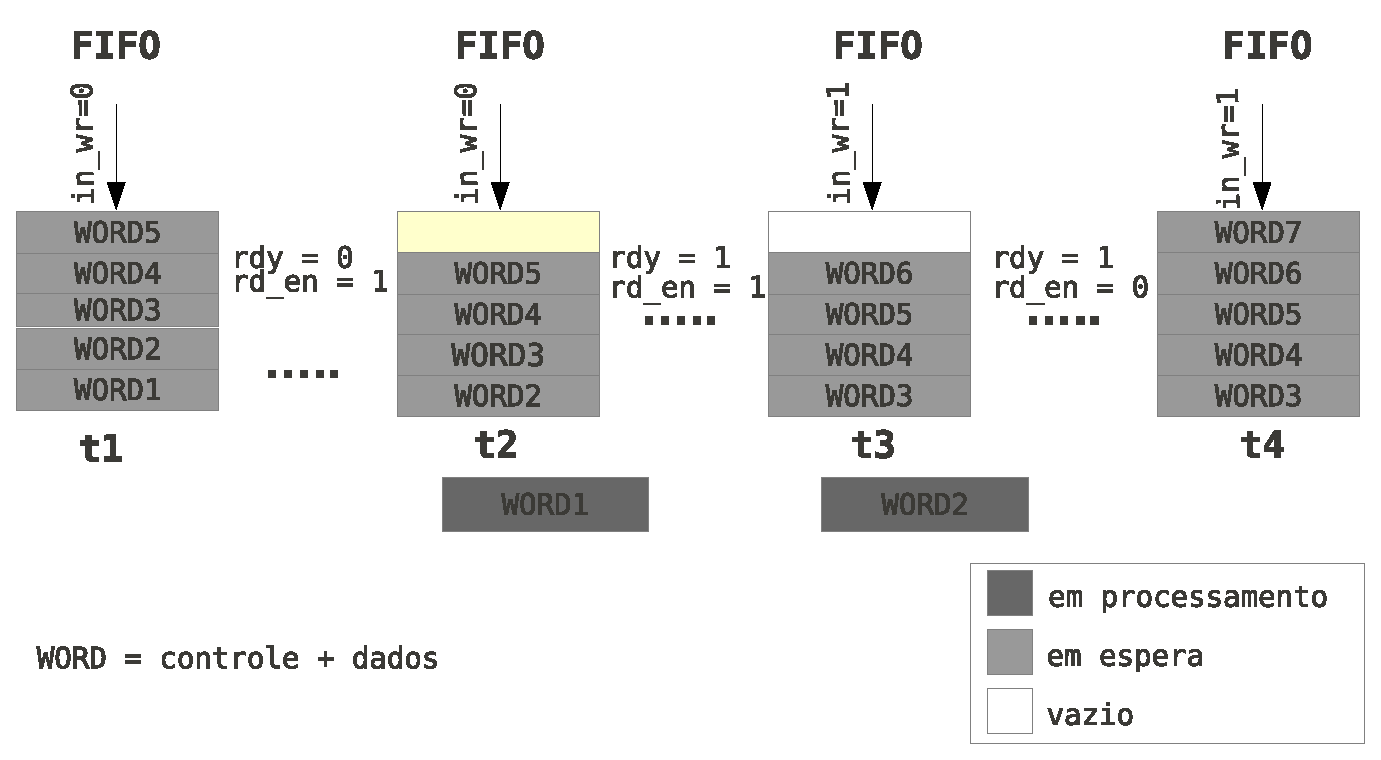
\includegraphics[scale=0.6,angle=0]{figures/modulos/fallthroughfifo.eps}
% \caption{Controle da fila de dados.}
% \label{fig:impl.fifo.msg}
% \end{figure}

\subsubsection{Máquina de estados}

Nosso \emph{firewall} implementa uma máquina de estados para verificar
se o pacote é IP e TCP.  Em caso positivo, a máquina de estados verifica
se a porta de destino deve ser filtrada e decide entre encaminhar ou
descartar o pacote.

Como todo o pacote é transmitido no barramento de encaminhamento com os
bits de controle zerados, nossa máquina de estado precisa manter
informação de qual palavra de 64~bits está sendo recebida.  Por exemplo,
como o cabeçalho IP e TCP somam pelo menos 40~bytes (56 bytes
contabilizando o cabeçalho Ethernet), o cabeçalho do pacote é recebido
ao longo de pelo menos cinco ciclos de relógio.  A
tabela~\ref{tab:impl.state.pktwords} mostra quais dados são transferidos
no barramento de encaminhamento a cada ciclo de relógio quando as linhas
de controle estão zeradas.

\begin{table}
\centering
\begin{tabular}{c|p{2.9cm}|p{2.9cm}|p{2.9cm}|p{2.9cm}|}
& \multicolumn{4}{c}{\ssf{in\_data}} \\
	Palavra & \multicolumn{1}{|c|}{\ssf{63:48}}     & \multicolumn{1}{|c|}{\ssf{47:32}}     & \multicolumn{1}{|c|}{\ssf{31:16}} & \multicolumn{1}{|c|}{\ssf{15:0}} \\ \hline
	1       & \multicolumn{3}{|l|}{Eth source addr} & Eth dest addr \\ \hline
	2       & \multicolumn{2}{|l|}{Eth dest addr}   & EtherType                             & IPver, HL, ToS \\ \hline
	3       & packet size                          & IP ID                                 & flags, frag                       & TTL, proto \\ \hline
	4       & checksum                             & \multicolumn{2}{|c|}{source IP}       & destination IP \\ \hline
	5       & destination IP                              & source port                          & destination port                         & seq. no. \\ \hline
	6       & seq. no.                             & \multicolumn{2}{|c|}{acknowledgement} & flags \\ \hline
	7       & adv. window                          & checksum                              & urgent ptr.                       & payload \\ \hline
	$\cdots$ & \multicolumn{4}{|l|}{payload} \\
\end{tabular}
\caption{Pacotes são encaminhados em palavras de 64 bits ao longo de
vários ciclos de relógio.  Na tabela um exemplo de pacote TCP.}
\label{tab:impl.state.pktwords}
\end{table}

\subsubsection*{Visão geral e atribuições padrão}

A figura~\ref{fig:impl.state.machine} mostra a máquina de estados do
nosso \emph{firewall}.  A ideia básica é receber o cabeçalho do pacote
para verificar se ele precisa ser descartado antes de transmiti-lo ao
próximo módulo.  Para receber e armazenar o cabeçalho do pacote
precisamos de uma fila de saída auxiliar, onde colocamos as palavras de
dados que já recebemos até decidir se devemos enviar o pacote para o
módulo seguinte ou descartá-lo.  A definição da fila de saída, mostrada
a seguir, é similar à definição da fila de entrada.

\begin{verilogcode}
   fallthrough_small_fifo #(
      ...
   ) output_fifo (
      .din           (out_fifo_din),   // Data in
      .wr_en         (out_fifo_wr),    // Write enable
      .rd_en         (out_fifo_rd_en), // Read the next word
      .dout          (out_fifo_dout),
      .full          (),
      .nearly_full   (out_fifo_nearly_full),
      .empty         (out_fifo_empty),
      .reset         (reset),
      .clk           (clk)
   );
\end{verilogcode}

A cada ciclo de relógio fazemos atribuições padrão que podem ser
sobrescritas dependendo do estado.  Em particular, deixamos a fila de
entrada travada, não escrevemos na fila de saída, e não repassamos dados
para o próximo módulo do \emph{pipeline}.  Também atribuímos os dados de
entrada da fila de saída aos dados retirados da fila de entrada.  Por
último, repassados ao próximo módulo no \emph{pipeline} os dados
retirados da fila de saída.

\begin{verilogcode}
    in_fifo_rd_en = 0;
    out_fifo_wr = 0;
    out_fifo_rd_en = 0;
    out_wr = 0;
    out_fifo_din = {in_fifo_ctrl, in_fifo_data};
    {out_ctrl, out_data} = out_fifo_dout;
\end{verilogcode}

\begin{figure}\centering
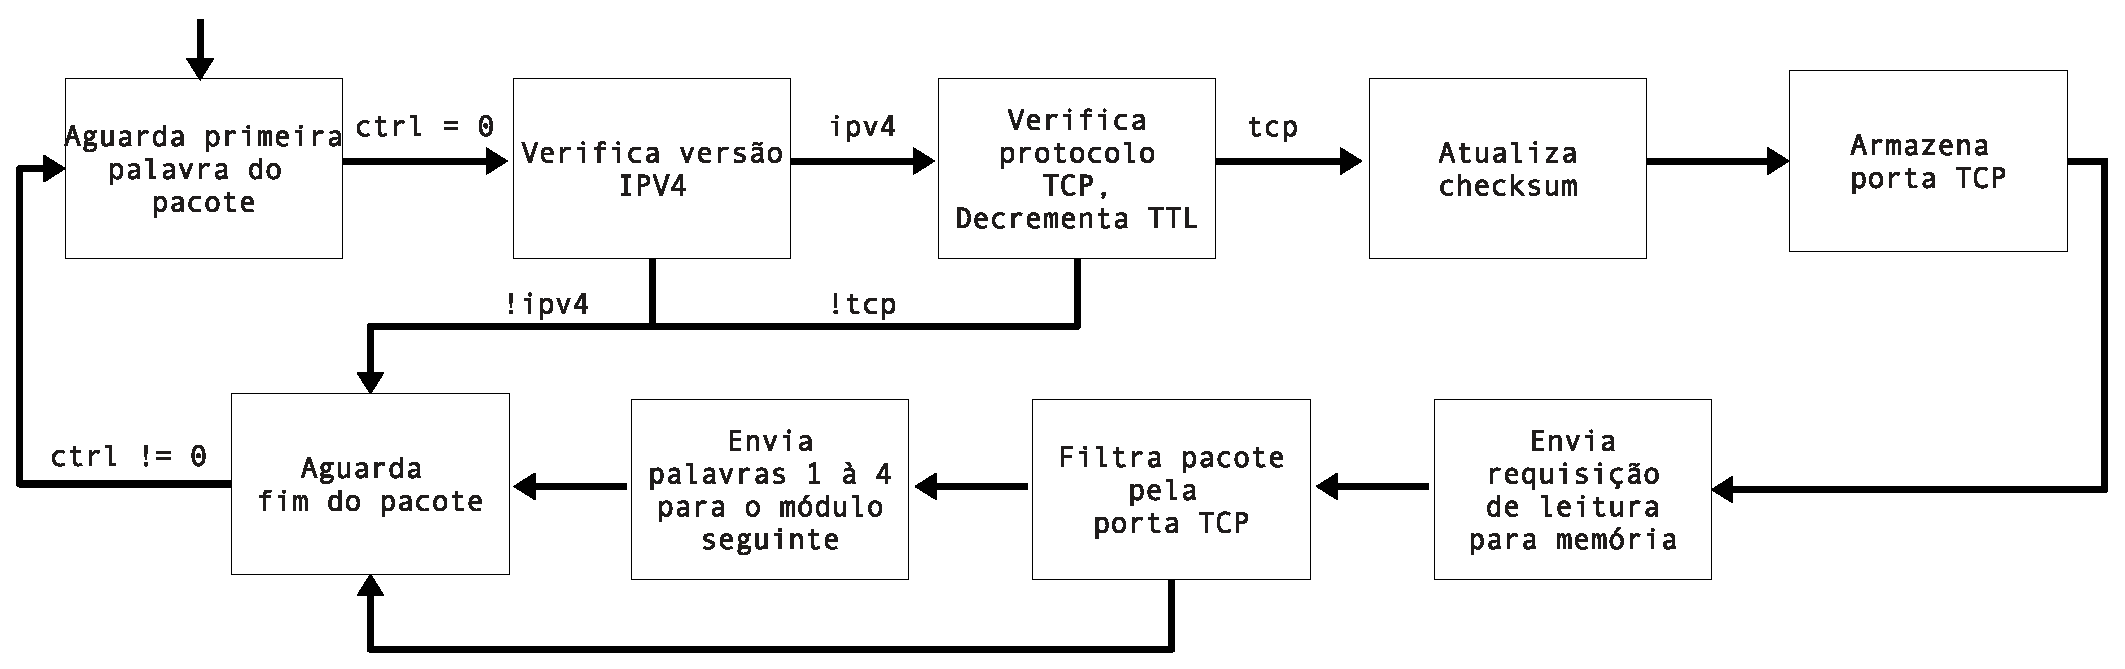
\includegraphics[scale=0.4]{figures/modulos/mestados.eps}
\caption{Máquina de estados do \emph{firewall}.}
\label{fig:impl.state.machine}
\end{figure}

Nossa máquina de estados atualiza todos os registradores a cada ciclo do
relógio.  Para cada registrador, temos um conjunto de linhas com o mesmo
nome e o sufixo \ssf{next}.  As linhas com sufixo \ssf{next} são
atribuídas aos respectivos registradores a cada ciclo do relógio.  Para
manter os valores nos registradores, inicializamos as linhas \ssf{next}
com o valor atual dos registradores e modificamos o valor das linhas
\ssf{next} em estados específicos quando necessário.

% \begin{minted}{verilog}
%       state_next = state;
%       save_1st_word_next = save_1st_word;
%       save_2nd_word_next = save_2nd_word;
%       save_3rd_word_next = save_3rd_word;
%       save_4th_word_next = save_4th_word;
%       dst_port_next = dst_port;
%       rd_0_req_next = 0;
%       num_TCP = num_TCP_next;
%       rd_0_addr_next = rd_0_addr;
%       drop_next = drop;
%       word_saved_next = word_saved;
% \end{minted}

\subsubsection*{Primeiro estado: esperando o início de pacotes}

O primeiro estado da nossa máquina de estados, \ssf{WAIT\_PACKET},
simplesmente espera o início do recebimento de um pacote, isto é, espera
as linhas de controle serem zeradas.  A implementação do primeiro
estado, mostrada abaixo, primeiro verifica se existe pacote a processar
e se o próximo módulo está pronto para receber pacotes verificando
\ssf{in\_fifo\_empty} e \ssf{out\_rdy}, respectivamente.  Se não há dado
a processar ou se o próximo módulo não está pronto para receber,
continuamos neste estado sem avançar as filas de entrada e saída (linha
12).  Se há dado a processar e o próximo módulo está pronto para
recebê-lo, nossa máquina de estados avança a fila ligando o sinal
\ssf{in\_fifo\_rd\_en} e grava os dados na fila de saída ligando
\ssf{out\_fifo\_wr}.  Se os bits de controle \ssf{in\_fifo\_ctrl} não
estiverem zerados, significa que ainda estamos recebendo metadados e o
início do pacote ainda não chegou.  Quando os bits de controle estiverem
zerados significa que acabamos de receber a primeira palavra de dados do
pacote (que contém o endereço MAC da origem,
tabela~\ref{tab:impl.state.pktwords}) e passamos para o segundo estado.

\begin{verilogcode}
  WAIT_PACKET: begin
     if (!in_fifo_empty && out_rdy) begin
        in_fifo_rd_en = 1;
        out_fifo_wr = 1;
        if(in_fifo_ctrl == 'h0) begin
           state_next = WORD2_CHECK_IPV4;
        end else begin
           state_next = WAIT_PACKET;
        end
     end
     else
        state_next = WAIT_PACKET;
  end
\end{verilogcode}


\subsubsection*{Segundo estado: verificação do protocolo de rede}

O segundo estado nosso \emph{firewall} processa a segunda palavra do
pacote e verifica se o pacote é um pacote IPv4.  Para isso verificamos
se o tipo do cabeçalho Ethernet (EtherType) é \ssf{0x0800}, que indica
um pacote IP, e se a versão do protocolo IP é \ssf{4}.\footnotemark{}
Em caso positivo, prosseguimos para o próximo estado para verificar se o
pacote é um pacote TCP.  Caso o pacote não seja um pacote IPv4 ele
deverá ser encaminhado pela rede sem ser filtrado.  Para encaminharmos o
pacote pulamos para o oitavo estado, \ssf{EMPTY\_OUT\_FIFO}, descrito
abaixo.

\footnotetext{Note que nosso \emph{firewall} não suporta VLANs (802.1Q).
Para tal seria necessário considerar o caso onde o EtherType é
\ssf{0x8100}.}

\begin{verilogcode}
  WORD2_CHECK_IPV4: begin
     if (!in_fifo_empty && out_rdy) begin
        if(in_fifo_data[31:16] != 16'h0800 ||
              in_fifo_data[15:12] != 4'h4) begin
           state_next = EMPTY_OUT_FIFO;
        end
        else begin
           in_fifo_rd_en = 1;
           out_fifo_wr = 1;
           state_next = WORD3_CHECK_TCP_TTL;
        end
     end
     else
        state_next = WORD2_CHECK_IPV4;
  end
\end{verilogcode}

\subsubsection*{Terceiro estado: verificação do protocolo de transporte}

No terceiro estado inspecionamos o cabeçalho IP para ver se o valor do
campo protocolo é \ssf{0x06}, que indica TCP.  Em caso negativo o pacote
é aceito: pulamos para o estado \ssf{EMPTY\_OUT\_FIFO} para enviarmos as
duas primeiras palavras mais metadados que foram armazenadas na fila de
saída (linha 9).  Note que, em caso negativo, a fila de entrada fica
bloqueada com a terceira palavra, que será transmitida após esvaziarmos
a fila de saída no estado \ssf{EMPTY\_OUT\_FIFO}.  Em caso positivo,
encaminhamos a terceira palavra para a fila de saída e passamos para o
próximo estado.

\begin{verilogcode}
  WORD3_CHECK_TCP_TTL: begin
     if (!in_fifo_empty && out_rdy) begin
        if(in_fifo_data[7:0] == 8'h06) begin
           in_fifo_rd_en = 1;
           out_fifo_wr = 1;
           state_next = WORD4_ADDR_CHKSUM;
        end
        else
           state_next = EMPTY_OUT_FIFO;
     end
     else
        state_next = WORD3_CHECK_TCP_TTL;
  end
\end{verilogcode}

\subsubsection*{Quarto estado: armazenamento dos endereços IP}

O quarto estado do \emph{firewall} armazena os dados da quarta palavra
do pacote temporariamente até verificarmos o número da porta de destino
no protocolo TCP no próximo estado.

\begin{verilogcode}
  WORD4_ADDR_CHKSUM: begin
     if (!in_fifo_empty && out_rdy) begin
        in_fifo_rd_en = 1;
        out_fifo_wr = 1;
        state_next = WORD5_TCP_PORT;
     end
     else
        state_next = WORD4_ADDR_CHKSUM;
  end
\end{verilogcode}

\subsubsection*{Quinto, sexto e sétimo estágios: verificando porta de
destino}

No quinto estado a fila de entrada contém a quinta palavra do pacote,
que possui o número da porta de destino do protocolo TCP.  Nós mantemos
as filas de entrada e saída travadas, armazenamos a porta de destino no
registrador \ssf{dst\_port} e avançamos para o próximo estágio.

\begin{verilogcode}
  WORD5_TCP_PORT: begin
     if (!in_fifo_empty && out_rdy) begin
        // in_fifo_rd_en and out_fifo_wr are zero by default
        dst_port_next = in_fifo_data[31:16];
        state_next = CHECK_RULES;
     end
     else
        state_next = WORD5_TCP_PORT;
  end
\end{verilogcode}

No sexto estágio mantemos as filas de entrada e saída travadas e
enviamos uma requisição de leitura da memória.  O endereço lido é
\ssf{SRAM\_PORTS\_ADDR}, que é definido igual a zero (primeira linha da
memória) e contém as portas de destino que estão bloqueadas.  Nós lemos
as portas bloqueadas da memória para ilustrar o acesso à memória SRAM e
porque as portas bloqueadas podem ser alteradas assincronamente pelo
usuário.  Na seção~\ref{sec:impl.mem} iremos detalhar o acesso à
memória.

\begin{verilogcode}
  CHECK_RULES: begin
     sram_rd_req_next = 1;
     sram_rd_addr_next = SRAM_PORTS_ADDR;
     state_next = CHECK_PORTS;
  end
\end{verilogcode}

Por último, o sétimo estágio espera a memória SRAM retornar os dados
verificando o valor de \ssf{rd\_vld}.  Esta espera é necessária pois a
SRAM demora alguns ciclos de relógio para retornar o dado requisitado.
Uma versão otimizada do nosso \emph{firewall} poderia realizar a
requisição de memória antes para evitar esta espera.  Se a porta de
destino for uma das portas bloqueadas, ligamos o registrador \ssf{drop}.
Independente da porta de destino passamos para o próximo estágio, onde a
fila de saída será esvaziada e os dados transmitidos para o próximo
módulo dependendo do valor do registrador \ssf{drop}.

\begin{verilogcode}
      CHECK_PORTS: begin
         if (rd_0_vld) begin
            if(sram_rd_data[15:0] == dst_port ||
                   sram_rd_data[31:16] == dst_port ||
                   sram_rd_data[47:32] == dst_port ||
                   sram_rd_data[63:48] == dst_port)
               drop_next = 1;
            else
               drop_next = 0;
            state_next = EMPTY_OUT_FIFO;
         end
         else
            state_next = CHECK_PORTS;
      end
\end{verilogcode}

\subsubsection*{Oitavo estágio: processando palavras armazenadas
temporariamente}

O oitavo estágio é responsável por processar os metadados e dados do
pacote armazenados temporariamente na fila de saída para o módulo
seguinte do \emph{pipeline}.  A cada ciclo de relógio processamos uma
palavra da fila de espera (linha 6).  Se o registrador \ssf{drop}
estiver desligado, enviamos uma palavra da fila de espera para o próximo
módulo (linha 7).  Se o registrador \ssf{drop} estiver ligado, retiramos
os dados da fila sem repassá-los ao módulo seguinte, efetivamente
descartando o pacote.  Quando a fila de espera estiver vazia pulamos
para o último estado onde enviamos o restante do pacote (a partir da
quinta palavra) para o próximo módulo diretamente da fila de entrada.

\begin{verilogcode}
      EMPTY_OUT_FIFO: begin
         if(!out_rdy)
            state_next = EMPTY_OUT_FIFO;
         else if(!out_fifo_empty) begin
            state_next = EMPTY_OUT_FIFO;
            out_fifo_rd_en = 1;
            out_wr = ~drop;
         end
         else
            state_next = PAYLOAD;
      end
\end{verilogcode}

\subsubsection*{Nono estágio: processando o conteúdo do pacote}

O nono e último estágio processa o resto do pacote a partir da fila de
entrada.  Os dados retirados da fila de entrada são repassados para o
próximo módulo dependendo do valor de \ssf{drop}.  Voltamos para o
primeiro estado quando detectamos o início do próximo pacote.
Detectamos o início do próximo pacote quando os bits de controle têm o
valor \ssf{IO\_QUEUE\_STAGE\_NUM}, do metadado adicionado pelas filas de
entrada quando o pacote é recebido na NetFPGA.  Note que assim que
detectamos o início do próximo pacote travamos a fila de entrada para
que a primeira palavra do pacote seja processada pelo primeiro estado do
\emph{firewall}.

\begin{verilogcode}
      PAYLOAD: begin
         if (!in_fifo_empty && out_rdy) begin
            {out_ctrl, out_data} = {in_fifo_ctrl, in_fifo_data};
            if(in_fifo_ctrl != `IO_QUEUE_STAGE_NUM)
                in_fifo_rd_en = 1;
                out_wr = ~drop;
                state_next = PAYLOAD;
            else begin
               in_fifo_rd_en = 0;
               out_wr = 0;
               drop_next = 0;            // reset drop register
               state_next = WAIT_PACKET;
            end
         end
         else
            state_next = PAYLOAD;
      end
\end{verilogcode}


